\documentclass{article}

% these packages let you do math
\usepackage{amsmath}
\usepackage{amssymb}

% we need these packages for fancy R tables
\usepackage{booktabs}
\usepackage{float}
\usepackage{colortbl}
\usepackage{xcolor}

% these packages play with the spacing/margins of the document. Uncomment the commands on lines 16 and 17 to see what they do.
\usepackage{a4wide}
\usepackage{setspace}
\usepackage{geometry}
\usepackage{parskip}
%\doublespacing
%\geometry{margin=1.5in}

% this package helps us with including images. Setting the graphics path makes it easier to refer to things in the \includegraphics command.
\usepackage{graphicx}
\graphicspath{ {../figures/} }

% make some hyperlinks using the \href command
\usepackage{hyperref}
\hypersetup{
    colorlinks=true,
    linkcolor=black,
    urlcolor=blue
}

% set the author, title, and date of the document. \maketitle adds it to the document.
\author{Colin McNally}
\title{Mean Months Incarcerated Paper}
\date{Spring 2022}

\begin{document}
\maketitle


\section{Graph of Average Months Incarcerated}

\begin{figure}[H]
    \begin{center}
        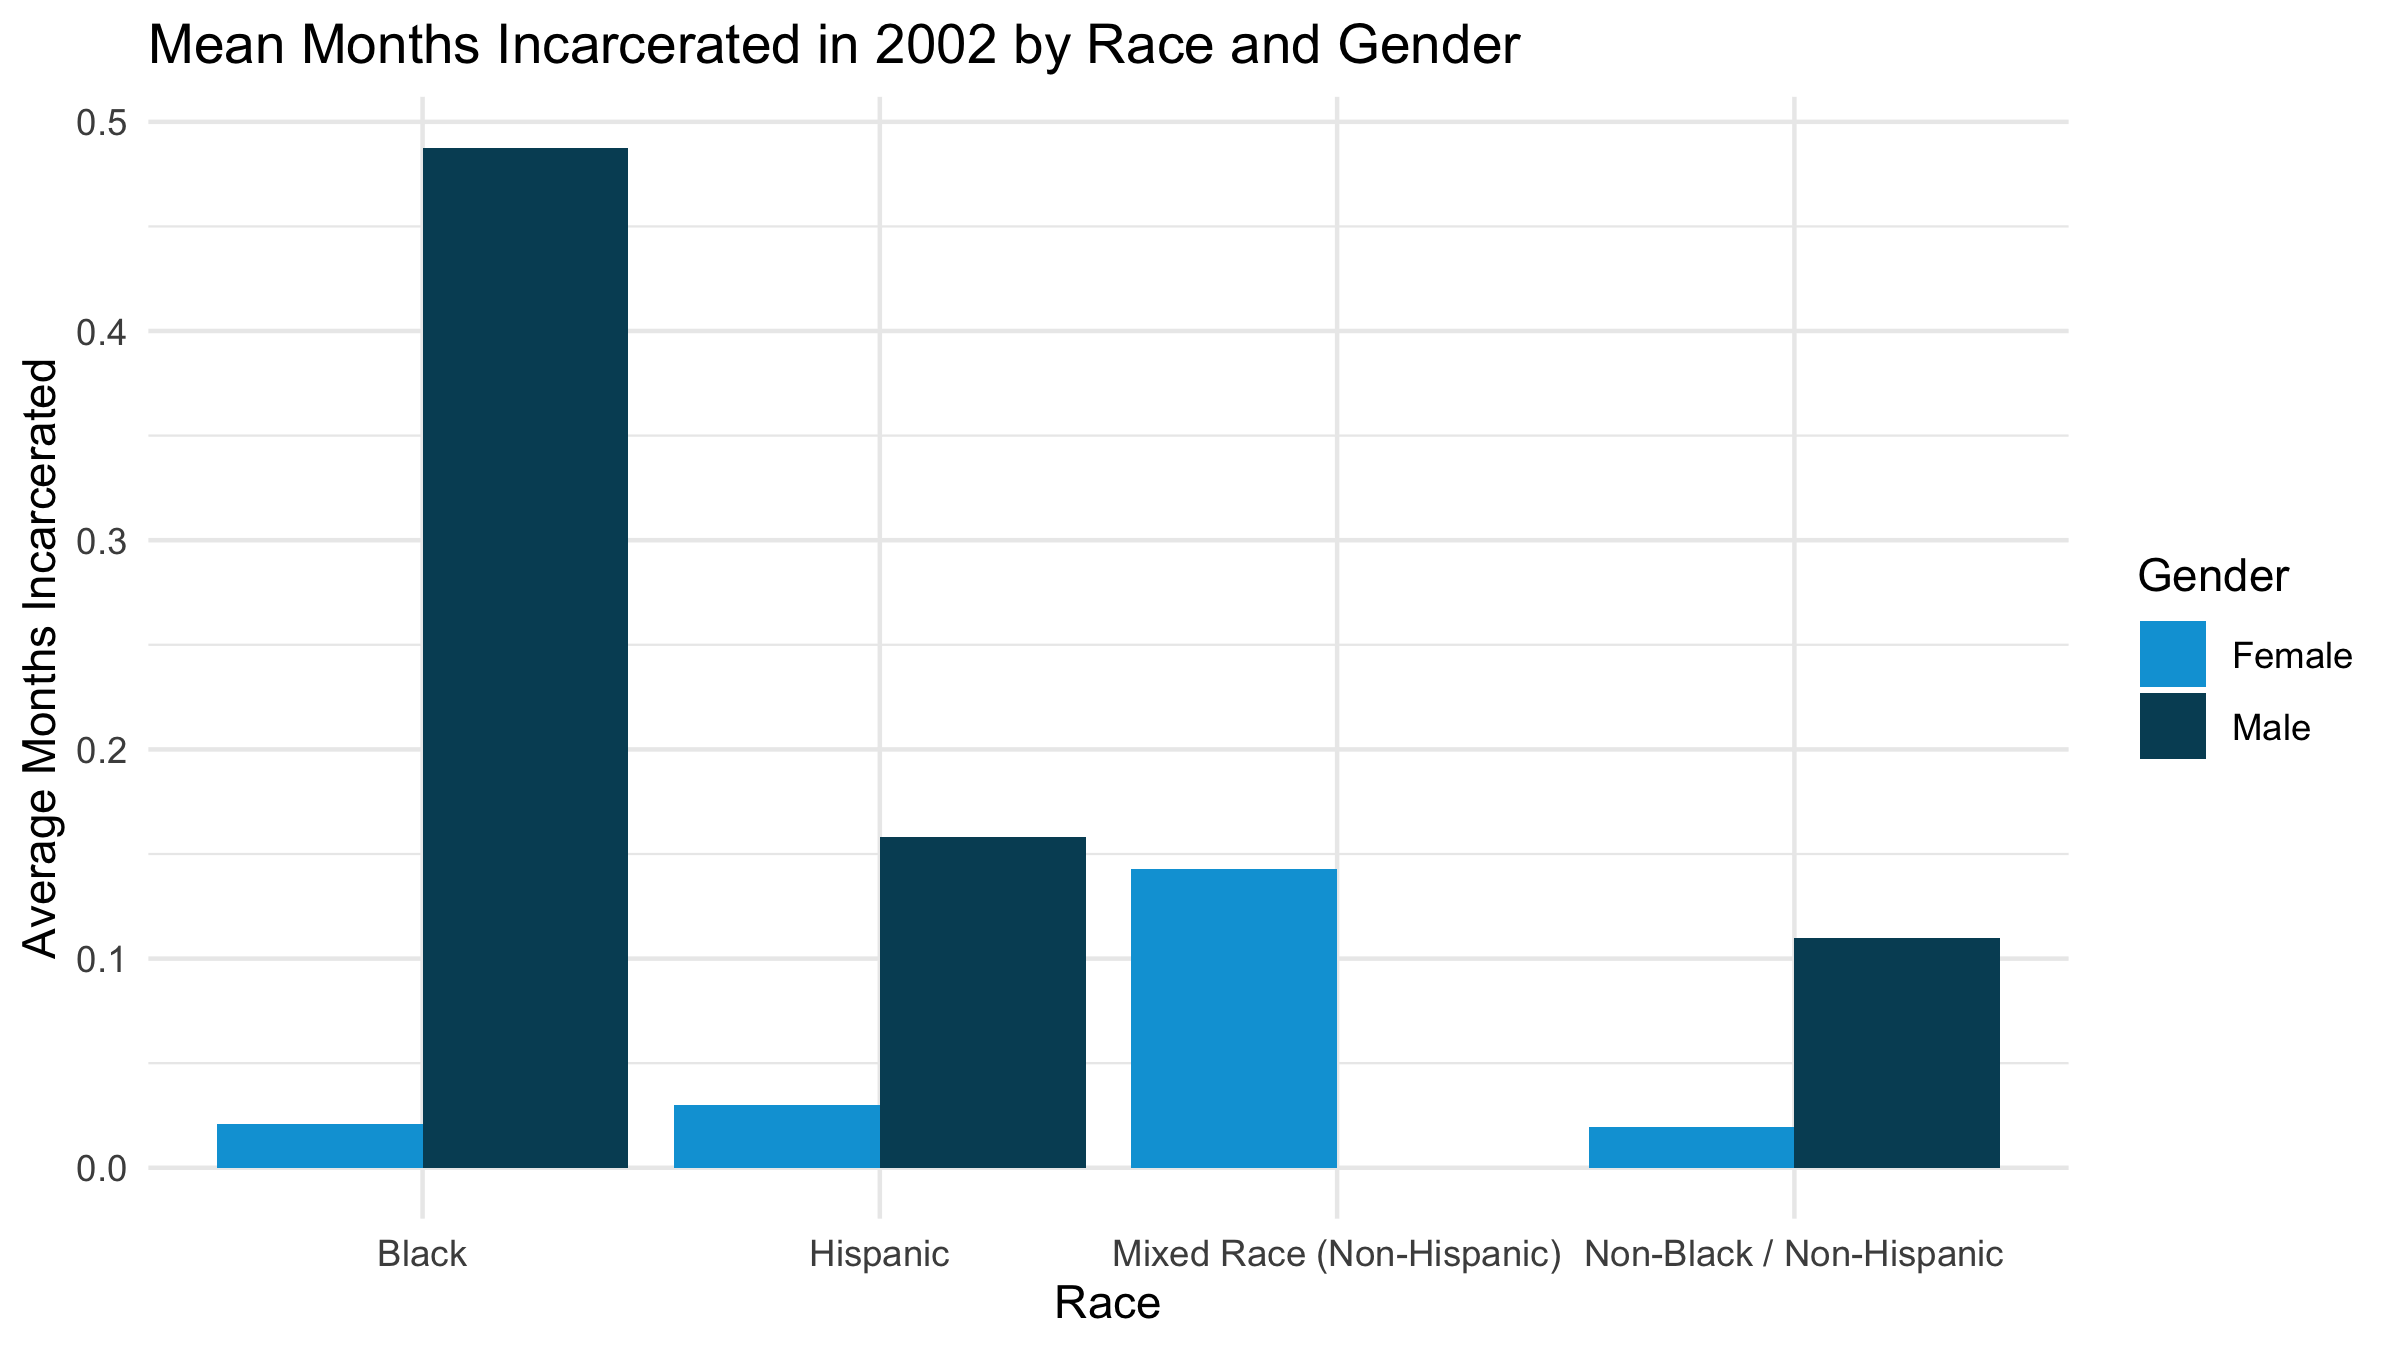
\includegraphics[width=.85\textwidth]{incarceration_by_racegender}
    \end{center}
    \caption{Mean Months Incarcerated in 2002 by Race and Gender (this is the LaTeX caption, not the ggplot title)}
    \label{fig:graph}
\end{figure}

In this graph we see that Black Men overwhelmingly are incarcerated for longer periods of time than any demographic. As well we see that most minority groups are incarcerated for longer periods of time than Non-Black/Non-Hispanic groups. Women in most categories are dwarfed by men of any race.

\newpage
\section{Mean Incarcerations Chart}
\begin{table}[H]

\caption{\label{tab:tab:summarystats}Mean Months Incarcerated in 2002 by Race and Gender}
\centering
\begin{tabular}[t]{lrrrr}
\toprule
Gender & Black & Hispanic & Mixed Race Non Hispanic & Non Black Non Hispanic\\
\midrule
\cellcolor{gray!6}{Female} & \cellcolor{gray!6}{0.0211268} & \cellcolor{gray!6}{0.0298013} & \cellcolor{gray!6}{0.1428571} & \cellcolor{gray!6}{0.0193192}\\
Male & 0.4876712 & 0.1579509 & 0.0000000 & 0.1099476\\
\bottomrule
\end{tabular}
\end{table}

Here we see that Women across all types race have a lower average amount of months incarcerated than Men of any race. Across races though Black Men are incarcerated for longer periods of time than any other subsection of data. Mixed Race Non Hispanic Women though have the highest mean incarceration lengths of any race for Women.

\newpage

\section{Regression of Race and Gender Variables}

\begin{table}[!htbp] \centering 
  \caption{Regression Output. Omitted category is Black Females.} 
  \label{tab:regression} 
\begin{tabular}{@{\extracolsep{5pt}}lc} 
\\[-1.8ex]\hline 
\hline \\[-1.8ex] 
 & \multicolumn{1}{c}{\textit{Dependent variable:}} \\ 
\cline{2-2} 
\\[-1.8ex] & Months Incarcerated in 2002 \\ 
\hline \\[-1.8ex] 
 Hispanic & $-$0.159$^{***}$ \\ 
  & (0.038) \\ 
  & \\ 
 Mixed Race (Non-Hispanic) & $-$0.174$^{**}$ \\ 
  & (0.083) \\ 
  & \\ 
 Non-Black / Non-Hispanic & $-$0.189$^{***}$ \\ 
  & (0.035) \\ 
  & \\ 
 Male & 0.194$^{***}$ \\ 
  & (0.022) \\ 
  & \\ 
 Constant & 0.155$^{***}$ \\ 
  & (0.026) \\ 
  & \\ 
\hline \\[-1.8ex] 
Observations & 8,621 \\ 
R$^{2}$ & 0.015 \\ 
Adjusted R$^{2}$ & 0.014 \\ 
Residual Std. Error & 1.019 (df = 8616) \\ 
F Statistic & 32.033$^{***}$ (df = 4; 8616) \\ 
\hline 
\hline \\[-1.8ex] 
\textit{Note:}  & \multicolumn{1}{r}{$^{*}$p$<$0.1; $^{**}$p$<$0.05; $^{***}$p$<$0.01} \\ 
\end{tabular} 
\end{table} 

We see here that being a Black Male instead of a Black Female increases the length of incarcerations by about 0.194 months in the year 2002. All other values of race see a decrease in expected length of incarceration compared to being Black. 


\end{document}
